\chapter{System Overview}

Multiple confined components serving specific purposes constitute the building blocks of the overall system, notably: \textit{the resource gatherer}, \textit{the resource clusterer}, \textit{the plant selector}, \textit{the ecosystem simulator} and \textit{the distribution analyser and reproducer}. The purpose of this chapter is to give an overview of the system, each component and how they fit together. To do so, an overview of each component is given separately. Each clearly stating the components purpose, required inputs and what it outputs. To conclude, figure \ref{fig:system_overview} gives an overview of the system, illustrating how the components fit together to make up the the overall system. \\

\section{Resource Gatherer}

Vegetation requires resources to grow, the amount of which uniquely identifies a given specie and associated it with given climate and locations on earth. Specifying this data is therefore essential to generating realistic virtual worlds in order to determine suitable vegetation and, subsequently, a suitable distribution thereof. The purpose of the resource gatherer is to determine, for each terrain vertex: \textit{Sun exposure}, \textit{Soil humidity}, \textit{Temperature} and the slope. Figure \ref{fig:system_overview_resource_gatherer} illustrates the output of the resource gatherer along with the user inputs required to generate them.

\begin{figure}
\center
	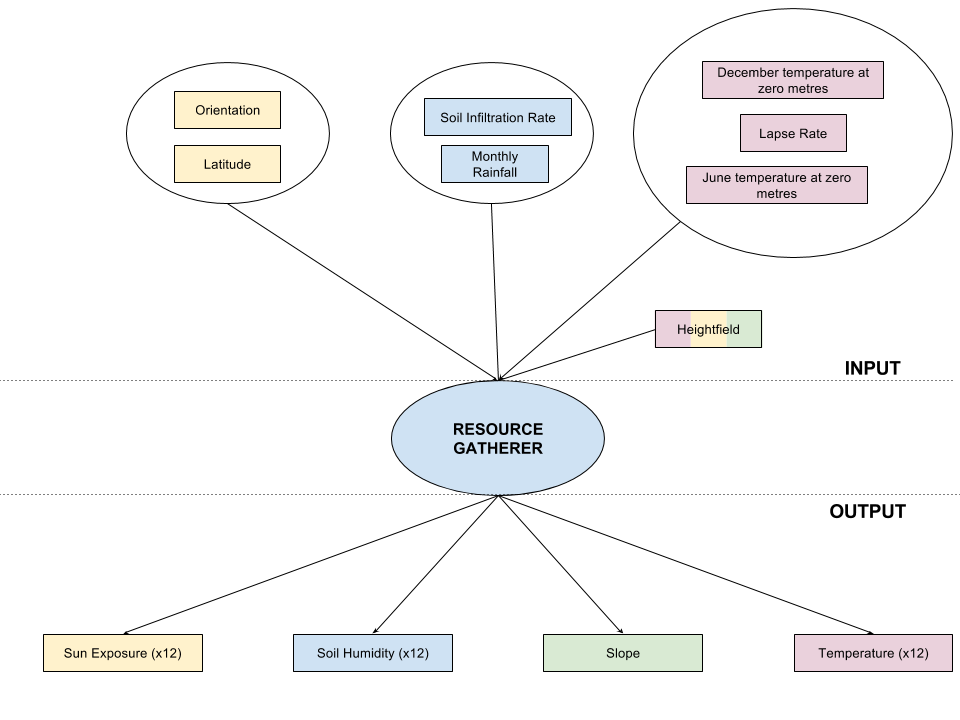
\includegraphics[width=\textwidth]{system_overview_resource_gatherer.png}
	\caption{ Resource gatherer overview with colour coding to correlate input with corresponding output.}	
	\label{fig:system_overview_resource_gatherer}
\end{figure}

\section{Resource Clusterer}

Determining a suitable plant distribution for each individual terrain vertex is infeasible due to the associated computational cost. To reduce the amount of plant distributions to calculate, K-means clustering is performed on the terrain to group together points with similar resource properties. The mean value of each cluster is used to determine suitable vegetation and distribution thereof. Figure \ref{fig:system_overview_resoure_clusterer} illustrates the input requirements and output of this component.

\begin{figure}
\center
	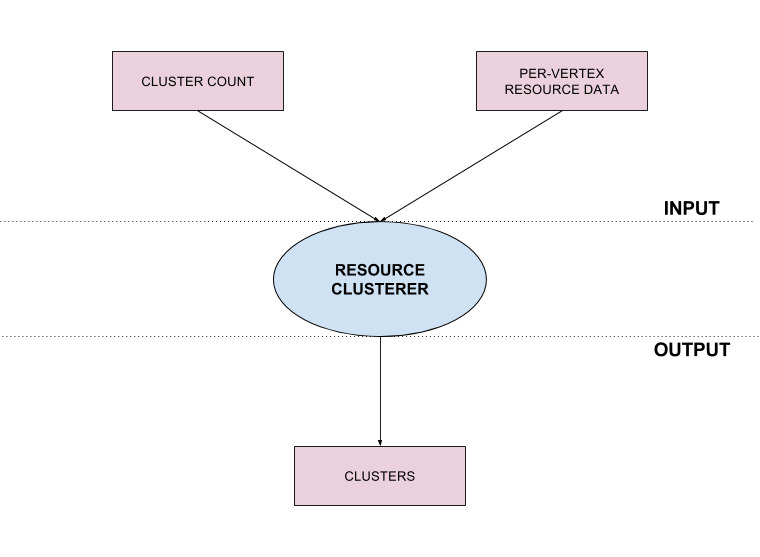
\includegraphics[width=\textwidth]{system_overview_resource_clusterer.png}
	\caption{ Resource clusterer overview.}	
	\label{fig:system_overview_resoure_clusterer}
\end{figure}

\section{Plant Selector}

Given the mean value of the individual clusters, the plant selector determines the plants which are able to survive on the terrain and calculates for each of them a suitability score. This score depicts how suited a specie is to each individual cluster and is illustrated to the user for informational purposes to facilitate the specie selection procedure. Figure \ref{fig:system_overview_plant_selector} shows the input requirements and outputs of this component.

\begin{figure}
\center
	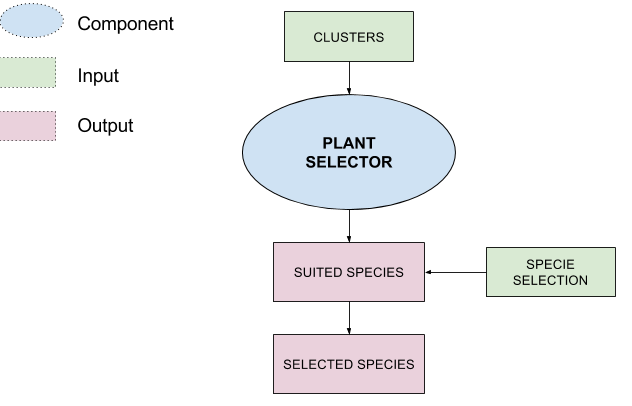
\includegraphics[width=\textwidth]{system_overview_plant_selector.png}
	\caption{ Plant selector overview.}	
	\label{fig:system_overview_plant_selector}
\end{figure}

\section{Ecosystem Simulator}

The ecosystem simulator is used to determine a valid plant distribution given a set of plant species and available resources. To so so, it simulates plants spawning, growing, battling and dying through time at monthly intervals on a hundred by hundred metre simulation area. Figure \ref{fig:system_overview_plant_selector} shows the input requirements and outputs of this component.

\begin{figure}
\center
	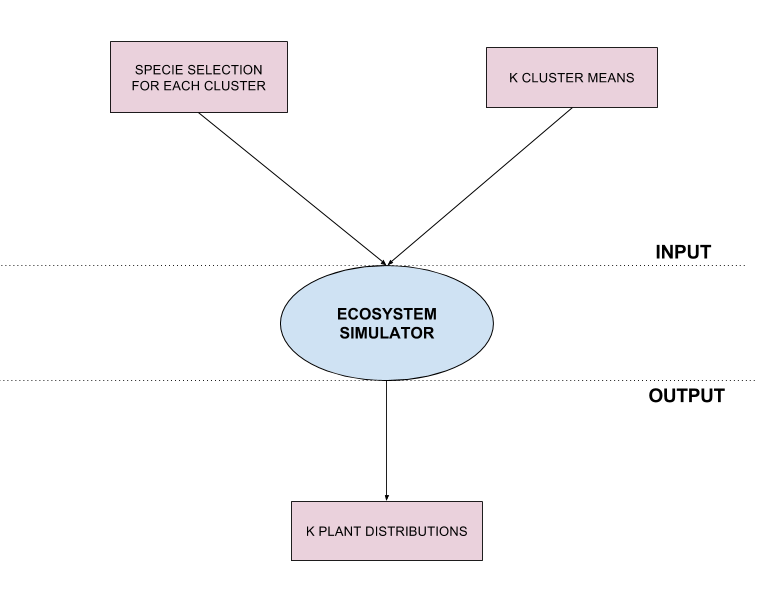
\includegraphics[width=\textwidth]{system_overview_ecosystem_simulator.png}
	\caption{ Ecosystem simulator overview.}	
	\label{fig:system_overview_plant_selector}
\end{figure}

\section{Distribution Analyser and Reproducer}

Because the ecosystem simulator is computationally expensive, the simulation area is restricted to ten thousand square metres (hundred by hundred metres). In order to place vegetation within clusters with a surface area larger than this, radial distribution analysis and reproduction is performed. This technique analyses the variation in plant density over distance of an input exemplar in order to generate pair correlation histograms which are subsequently used to reproduce distributions matching the characteristics of the input exemplar. Because the reproduction is much less computationally costly than the ecosystem simulator, it is possible to efficiently produce distributions covering much larger areas. Figure \ref{fig:system_overview_distribution_analyser_and_reproducer} shows the input requirements and outputs of this component.

\begin{figure}
\center
	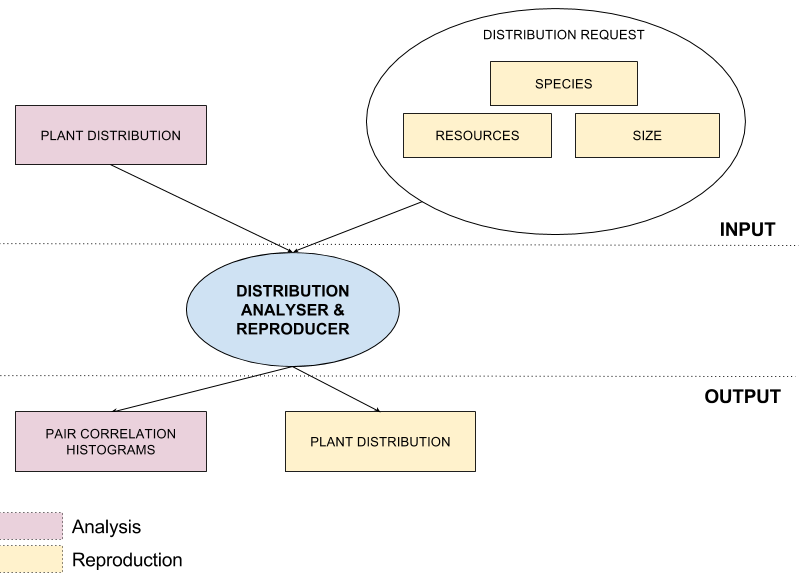
\includegraphics[width=\textwidth]{system_overview_radial_distribution_analyzer_and_reproducer.png}
	\caption{ Distribution analyser and reproducer overview.}	
	\label{fig:system_overview_distribution_analyser_and_reproducer}
\end{figure}

\begin{figure}
\center
	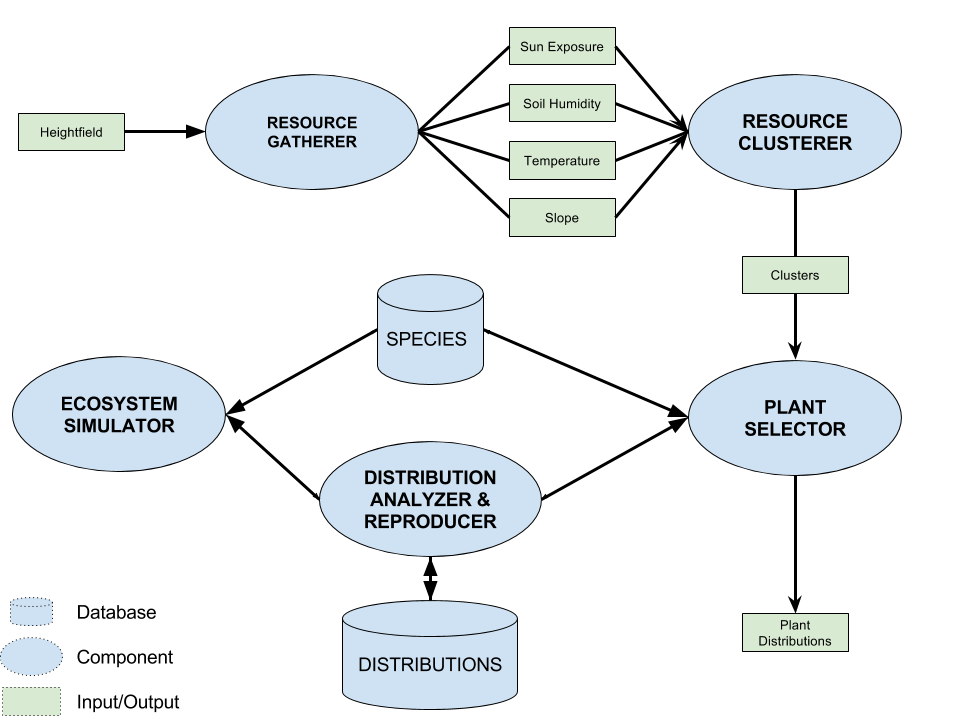
\includegraphics[width=\textwidth]{system_overview.png}
	\caption{ System overview}	
	\label{fig:system_overview}
\end{figure}
